\documentclass[UTF-8,twoside,c5size]{ctexart}
\usepackage[dvipsnames]{xcolor}
\usepackage{amsmath}
\usepackage{amssymb}
\usepackage{geometry}
\usepackage{listings}
\usepackage{setspace}
\usepackage{xeCJK}
\usepackage{ulem}
\usepackage{pstricks}
\usepackage{pstricks-add}
\usepackage{bm}
\usepackage{mathtools}
\usepackage{breqn}
\usepackage{mathrsfs}
\usepackage{esint}
\usepackage{textcomp}
\usepackage{upgreek}
\usepackage{pifont}
\usepackage{tikz}
\usepackage{circuitikz}
\usepackage{caption}
\usepackage{tabularx}
\usepackage{array}
\usepackage{pgfplots}
\usepackage{multirow}
\usepackage{pgfplotstable}
\usepackage{mhchem}
\usepackage{graphicx}
\usepackage[cache=false]{minted}
\usepackage{multicol}

\newcolumntype{Y}{>{\centering\arraybackslash}X}
\geometry{a4paper,centering,top=1.27cm,bottom=2.54cm,left=2cm,right=2cm}
\graphicspath{{figures/}}
\pagestyle{plain}
\captionsetup{font=small}

%\CTEXsetup[name={,.}]{section}
\CTEXsetup[format={\raggedright\heiti\noindent\zihao{-3}},numberformat={\bfseries}]{section}
\CTEXsetup[format={\raggedright\heiti\zihao{4}},numberformat={\bfseries}]{subsection}
\CTEXsetup[format={\raggedright\heiti\quad\zihao{-4}},numberformat={\bfseries}]{subsubsection}
\CTEXsetup[format={\raggedright\heiti\qquad},numberformat={\bfseries}]{paragraph}
\CTEXsetup[beforeskip=1.0ex plus 0.2ex minus .2ex, afterskip=1.0ex plus 0.2ex minus .2ex]{paragraph}

\CTEXsetup[format={\raggedright\heiti\qquad},numberformat={\bfseries},name={\bfseries(,)}]{subparagraph}
\CTEXsetup[beforeskip=1.0ex plus 0.2ex minus .2ex, afterskip=1.0ex plus 0.2ex minus .2ex]{subparagraph}
\renewcommand\thefootnote{\ding{\numexpr171+\value{footnote}}}

\setstretch{1.5}

\setCJKfamilyfont{boldsong}[AutoFakeBold = {2.17}]{SimSun}
\newcommand*{\boldsong}{\CJKfamily{boldsong}}
%\DeclareMathOperator\dif{d\!}
\newcommand*{\me}{\mathop{}\!\mathrm{e}}
\newcommand*{\mpar}{\mathop{}\!\partial}
\newcommand*{\dif}{\mathop{}\!\mathrm{d}}
\newcommand*{\tab}{\indent}
\newcommand*{\mcelsius}{\mathop{}\!{^\circ}\mathrm{C}}
\renewcommand*{\Im}{\mathrm{Im}\,}

\setcounter{secnumdepth}{5}

\renewcommand\arraystretch{1.5}
\renewcommand\thesubparagraph{\arabic{subparagraph}}

\lstset{
	backgroundcolor=\color[RGB]{245,245,245},
	keywordstyle=\color{blue}\bfseries,
	basicstyle=\small\ttfamily,
	commentstyle=\itshape\color{olive},
	numberstyle=\ttfamily,
	tabsize=4,
	breaklines=true
}

\setminted{style=manni,fontsize=\small,breaklines=true}

\begin{document}
	\begin{center}
		\heiti\zihao{-2}
		实验\textbf{10 $ \bm\sim $ 12}报告
	\end{center}

	\begin{table*}[!h]
		\raggedleft
		\zihao{-4}
		\begin{tabular}{ccc}
			{\heiti 学号} & {2019K8009929019} & {2019K8009929026} \\
			{\heiti 姓名} & 桂庭辉 & 高梓源 \\
			{\heiti 箱子号} & \multicolumn{2}{c}{44}
		\end{tabular}
	\end{table*}
	
	\section{实验任务}
	
	本次实验目的是为CPU适配指令和数据RAM,大致可分为两个主要阶段:CPU内部调整按照类SRAM时序调整指令和数据发送接收状态;CPU与外部采用AXI接口设计,经过“桥片”将内部SRAM信号调整至AXI信号以便发送至外部RAM。
	
	\section{实验设计}	
	
	\subsection{总体设计思路}
	
	在CPU内部将数据的请求和接收拆分开,使用\texttt{pre_if}和\texttt{es}两级流水级发送数据请求信号,在\texttt{if}和\texttt{ms}两级准备好数据的接收即可。正常情况比较容易考虑,思路可以采取状态机或者直接使用控制信号交互关系进行建模。异常处理和跳转需要单独考虑,结合时序推出信号应有状况,而后引入其他中间量协调处理。
	
	CPU外部的SRAM-AXI转换可以使用FIFO或状态机,本组采用后者,利用状态机状态对控制信号进行赋值调整,简易直观的思路,并且根据AXI协议的特点(高效性)为密集的读写任务增加了事务处理的计数信号,以此与状态机形成互补。
	
	\subsection{重要模块设计:\texttt{pre_if}流水级}
	
	\subsubsection{功能描述}
	
	作为单独拉出的伪流水级,承担原先\texttt{fs}级一半功能,即发出取指请求,并只会将有效指令地址送入\texttt{fs}级。
	
	\subsubsection{工作原理}
	
	首先,该流水级完成的核心功能为对\texttt{inst_sram}请求信号的赋值,而后根据\texttt{inst_sram_addr_ok}信号返回(即决定请求是否被接收)将这一流水级设置为可流向下一级,若下一级接收则更新这一流水级的指令,发起新一拍取指操作。
	
	\subsubsection{接口定义}
	
	作为单独一级伪流水,实际上和正常流水级采取相同的控制信号完成流水的传递。因为取指操作需要考虑异常处理和转移指令,还需加上相关信号。
	
	\begin{table}[!h]
		\centering
		\caption{\texttt{pre_if}流水级模块接口}
		\begin{tabularx}{\textwidth}{|c|c|c|Y|}
			\hline
			\textbf{名称} & \textbf{方向} & \textbf{位宽} & \textbf{描述} \\
			\hline
			\texttt{clk} & \textsc{In} & 1 & 时钟信号 \\
			\hline
			\texttt{rst} & \textsc{In} & 1 & 复位信号,高电平有效 \\
			\hline
			\texttt{fs_allowin} & \textsc{In} & 1 & \texttt{fs}流水级是否允许流入 \\
			\hline
			\texttt{pfs_to_fs_bus} & \textsc{Out} & 32 &  \texttt{pfs}正确指令已经取指,流入下一级\\
			\hline
			\texttt{pfs_to_fs_valid} & \textsc{Out} & 1 & 当前\texttt{pfs}级是否可以流入下一级 \\
			\hline
			\texttt{br_bus} & \textsc{In} & 35 & 从\texttt{id}级前递的跳转相关信号 \\
			\hline
			\texttt{inst_sram_req} & \textsc{Out} & 1 & 发起取指请求 \\
			\hline
			\texttt{inst_sram_wr} & \textsc{Out} & 1 & 指令RAM写或读,恒为0,读 \\
			\hline
			\texttt{inst_sram_size} & \textsc{Out} & 2 & 请求的数据大小,恒为\texttt{2'b10},代表4字节 \\
			\hline
			\texttt{inst_sram_wstrb} & \textsc{Out} & 4 & 写窗口,恒为0 \\
			\hline
			\texttt{inst_sram_addr} & \textsc{Out} & 32 & 请求地址,为nextpc值 \\
			\hline
			\texttt{inst_sram_wdata} & \textsc{Out} & 32 & 写数据,恒为0 \\
			\hline
			\texttt{inst_sram_addr_ok} & \textsc{In} & 1 & 高电平表示取指请求已被成功接收 \\
			\hline
			\texttt{inst_sram_data_ok} & \textsc{In} & 1 & 高电平表示指令已成功返回 \\
			\hline
			\texttt{wb_exc} & \textsc{In} & 1 & 出现异常,清空流水线 \\
			\hline
			\texttt{wb_ertn} & \textsc{In} & 1 & 异常返回,重新回到出发异常地址继续执行 \\
			\hline
			\texttt{exc_entry} & \textsc{In} & 32 & 异常处理入口 \\
			\hline
			\texttt{exc_retaddr} & \textsc{In} & 32 & 异常返回地址 \\
			\hline
		\end{tabularx}
	\end{table}

	\subsubsection{取指请求的发起}
	
	由其余取指请求信号的赋值都较为简单,在上表已列出,这里就较为复杂的取指请求简要说明。
	
	正常情况下,若当前\texttt{pfs}级有效、\texttt{fs}级可进入(采取简单做法,避免不必要的麻烦,但牺牲了些许性能)时将取指请求拔高,发起请求即可。
	
	在早期尝试过程中,发现若\texttt{pfs}不等待\texttt{fs_allow_in}拔高就发请求,而后使用缓冲数组将请求结果暂存并不能解决问题,因为情况很复杂,不能确定之后流水级的接收情况,尤其是在访存指令执行期间需要阻塞一段时间,使得完成“{\kaishu 在\texttt{fs}级被阻塞时使用缓冲暂存返回的指令}”的目标需要极端情况无限大的缓冲区,这便不确定了。于是最后还是采用简单的做法,保证正确性。
		
	在Lab10的SRAM接口处理中,若当前请求未被接收是可以改变请求内容的,而在Lab11$\sim$Lab12中由于AXI协议及笔者设计的状态机,一旦试图发起请求,该请求一定会被接收,因此异常(包含例外和跳转,下同)情况下可以采取不同的方式。Lab10中一旦发生异常,可以检查是否已经接收,若未接收,则可以直接替换掉取指的地址,这样等到接收该申请的时候已经自动变成正确指令取指了;而若该次取指已经被接收,则需要将其无效掉,处理方式按照下面Lab11$\sim$Lab12的方式即可。
	
	在Lab11$\sim$Lab12中,因为之后会讲的AXI转接的状态机设计,一旦\texttt{inst_sram_req}拉高,一定会保持在等待接收状态,这时所有信号由状态机决定赋值,并不会根据\texttt{pfs}的取指请求改变而改变,因此情况变得简单:\textsl{错误的取指请求一定会被接受},但实际上还要分情况:是否发起过取指请求,若错误指令由于\texttt{fs_allowin}的阻塞并未发请求,则不必取消,改变请求后继续按照正常发请求即可;若已经发起过取指请求,则必须要无效掉该请求及其返回指令,简单的方式是在这种情况下取消\texttt{pfs_ready_go},由于组合逻辑设计来推导,这等价于取消\texttt{pfs_to_fs_valid},于是接下去\texttt{fs_valid}无效,\texttt{fs_to_ds_valid}无效,这样即使错误指令被返回,\texttt{inst_sram_data_ok}拉高也不会被\texttt{fs}视为有效指令而流向下一级,这部分代码逻辑如下,感兴趣读者可以稍作思考:
	
    \begin{minted}{verilog}
    // pre_if stage
    // when we need to reflush, inst_sram_req became low
    assign inst_sram_req = ~reset && pfs_valid && fs_allowin & ~(pfs_reflush);
    // pfs not ready to go
    assign pfs_ready_go = (inst_sram_addr_ok && inst_sram_req) && ~(((wb_ertn_r || wb_exc_r || br_stall_r) && pfs_reflush) || wb_exc || wb_ertn || br_stall);
    // so it's not valid
    assign pfs_to_fs_valid = pfs_valid && pfs_ready_go;
    // IF stage
    // then fs_valid low (fs allow in)
    always @(posedge clk) begin
        if (reset) begin
            fs_valid <= 1'b0;
        end
        else if (fs_allowin) begin
            fs_valid <= pfs_to_fs_valid;
        end
    end
    // even if inst_sram_data_ok, fs to ds is not valid, wrong instruction cancelled
    assign fs_to_ds_valid =  fs_valid && fs_ready_go && ~fs_inst_cancel;
    \end{minted}
		
	上面代码中\texttt{pfs_reflush}信号正是刻画了这种需要取消的情况,在Lab10和Lab11$\sim$Lab12中,可以按照如下方式赋值:
	    
    \begin{multicols}{2}
    Lab10
    \begin{minted}{verilog}
    if(reset) begin
        pfs_reflush <= 1'b0;
    end else if(inst_sram_addr_ok_r
        && (wb_exc | wb_ertn | (~br_stall && br_taken)) begin
        pfs_reflush <= 1'b1;
    end else if(inst_sram_data_ok) begin
        pfs_reflush <= 1'b0;
    end
    \end{minted}
        
    \hfill
    
    Lab11$\sim$Lab12
    \begin{minted}{verilog}
    if(reset) begin
        pfs_reflush <= 1'b0;
    end else if(inst_sram_req
        && (wb_exc | wb_ertn | (br_stall && inst_sram_addr_ok))) begin
        pfs_reflush <= 1'b1;
    end else if(inst_sram_data_ok) begin
        pfs_reflush <= 1'b0;    
    end
    \end{minted}
    
    \hfill
    
    \end{multicols}
	
	左边即若已接收后收到必须清理流水线的信号时拉高,右边即若收到清流水信号,但已经发起请求,注意\texttt{branch}操作有些特殊,因为\texttt{stall}时也可能发起请求,但不一定是错误的,我们可以统一处理,若未收到接收信号令其继续发请求,若收到信号去清这一拍,等到\texttt{stall}结束,根据跳转有效/无效重新发请求。恢复的条件是错误请求的指令返回,即\texttt{inst_sram_data_ok}拉高,此时一切将正常。
	
	为了配合清流水以及在之后恢复正常取指操作,异常信号都需要用\texttt{reg}拉住,直到正常时取指请求被接收时恢。用处在于利用\texttt{nextpc}取到正确指令提供稳定的选择。因为在整个异常到来到正确请求接收的过程中都需要统一的正确地址,因此需要一直拉住。
	
    \begin{minted}{verilog}
    assign nextpc   = wb_exc   ? exc_entry   : wb_exc_r   ? exc_entry_r   :
                      wb_ertn  ? exc_retaddr : wb_ertn_r  ? exc_retaddr_r :
                      br_taken_r ? br_target_r : br_taken && !br_stall) ? br_target   :
                                 seq_pc;
    \end{minted}
	
	\subsection{模块设计更新:\texttt{if}流水级}
	
	\subsubsection{功能描述}
	
	这里主要把\texttt{if}流水级的取指请求移到了\texttt{pre_if}级,而后只需要在此考虑取指接收的情况。思路较为简单,按照讲义描述,若有效指令返回时\texttt{ds}可以进入,则直接将\texttt{inst_sram_data}作为结果送入\texttt{ds};若译码级被阻塞,则设置缓冲区存放取回的指令,在译码级可进入的情况下优先选择缓冲区中的数据。
	
	\subsubsection{接口定义}
	
	\texttt{pre_if}模块更新接口如下,之前已有接口不再赘述,此外,由于取指请求和地址计算操作移到了\texttt{pre_if},这里不再需要\texttt{branch}信号的接入:
	
	\begin{table}[!h]
	\begin{center}
		\caption{\texttt{if}流水级模块更新接口}
		\begin{tabularx}{\textwidth}{|c|c|c|c|Y|}
			\hline
			\textbf{名称} & \textbf{方向} & \textbf{更新操作} & \textbf{位宽} & \textbf{描述} \\
			\hline
			\texttt{inst_sram_data_ok} & \textsc{In} & $+$ & 1 & 高电平表示指令已成功返回 \\
			\hline
			\texttt{inst_sram_data} & \textsc{In} & $+$ & 32 & 取回的指令 \\
			\hline
			\texttt{br_bus} & \textsc{In} & $-$ & 35 & 跳转前递信号 \\
			\hline
		\end{tabularx}
	\end{center}
	\end{table}

	\subsubsection{取指结果的返回}

	根据前面功能描述,这里的设计很显而易见,当\texttt{inst_sram_data_ok}拉高时有三种情况:1)\texttt{ds}可以进入,这是正确指令;2)\texttt{ds}被阻塞,这是正确指令;3)异常处理触发,这是错误指令。对于正确指令的返回,在1的情况下可以直接将\texttt{fs_ready_go}拉高,导致\texttt{fs_to_ds_valid}有效,\texttt{ds}可以进入,指令流向译码级;第二种情况要令\texttt{fs_inst_buff_valid}为高,同时将指令存入\texttt{fs_inst_buff}。
	
	第三种情况中需要考虑连续两条指令,即正在取指的指令和\texttt{pre_if}级以及发起过请求的指令,对于正在取指的指令在前面\texttt{pre_if}已经分析过,不会产生破坏影响;而后由异常处理的需求,在异常处理拉高的时候,所有流水线都需要清空本纪,方法是将去往下一级的\texttt{valid}信号拉低,使其无效即可,这样下一级也不会接受和处理当前指令。
	
	对于\texttt{fs}级的情况,简单的做法仍然是利用\texttt{reg}信号将错误指令和\texttt{pre_if}级取消的请求结果的ok信号抹除,即\texttt{fs_to_ds_valid}拉低。这里\texttt{reg}信号的处理与其他所有流水级一致,在此说明而后面跳过,即在异常触发的时候拉高,直到前面一级流水传递进来新的有效指令为止,即前一级前往本级\texttt{valid}信号拉高。
	
	\subsection{模块设计更新:\texttt{ds}流水级}
	
	\subsubsection{功能描述}
	
	针对访存指令请求数据RAM的服务,在\texttt{ds}流水级添加数据RAM请求信号,并且调整相关流水线控制逻辑。
	
	\subsubsection{接口定义}
	
	更新的接口设计如下:
	
	\begin{table}[!h]
		\begin{center}
			\caption{\texttt{ds}级更新接口}
			\begin{tabularx}{\textwidth}{|c|c|c|c|Y|}
				\hline
				\textbf{名称} & \textbf{方向} & \textbf{更新操作} & \textbf{位宽} & \textbf{描述} \\
				\hline
				\texttt{data_sram_req} & \textsc{Out} & $+$ & 1 & 发起数据RAM事务请求 \\
				\hline
				\texttt{data_sram_wr} & \textsc{Out} & $+$ & 1 & 数据RAM写或读,\texttt{load}为0,\texttt{store}为1 \\
				\hline
				\texttt{data_sram_size} & \textsc{Out} & $+$ & 2 & byte为2'b0,half word为2'b1,word为2'b10 \\
				\hline
				\texttt{data_sram_wstrb} & \textsc{Out} & $+$ & 4 & 写窗口,根据取指地址及数据大小确定 \\
				\hline
				\texttt{data_sram_addr} & \textsc{Out} & $+$ & 32 & 请求地址,来自\texttt{alu_result} \\
				\hline
				\texttt{data_sram_wdata} & \textsc{Out} & $+$ & 32 & 写数据 \\
				\hline
				\texttt{data_sram_addr_ok} & \textsc{In} & $+$ & 1 & 高电平表示请求已被成功接收 \\
				\hline
				\texttt{ms_to_es_ls_cancel} & \textsc{In} & $+$ & 1 & 若\texttt{ms}出现异常,\texttt{es}的访存操作需要立即取消 \\
				\hline
			\end{tabularx}
		\end{center}
	\end{table}

	\subsubsection{数据RAM的请求信号}
	
	正常情况下十分简单,只需要在\texttt{ds}译码得出是\texttt{load, store}指令的时候,且\texttt{ms_allow_in}的时候发起请求即可。
	
	事实上,针对后一条件,在Lab10 SRAM接口和无延迟的AXI接口中问题不大,但是在复杂随机条件下,会出现有趣的问题,基于AXI协议的高效性,AXI读通道和写通道分开处理,因此它我们二者之间的关系无从知晓,也就是会可能出现以下情况:若连续3条指令为\texttt{store, load, store},那么AXI的slave端返回高电平顺序有可能是:\{\texttt{rvalid, bvalid, bvalid}\},\{\texttt{bvalid, rvalid, bvalid}\},\{\texttt{bvalid, bvalid, rvalid}\}。此时如何判断\texttt{data_sram_data_ok}何时拉高才能使读写结果对应到正确的读写指令上?照这个思路,只要是读写指令间隔出现,就需要无穷大不确定数量的缓冲区存储先前到达的状态,并且对于每个读写事务要标记先后次序,会非常复杂。因此简单考虑,只需要让读写严格按照次序进行,读结果返回之后才能写,写同理。
	
	对于异常,这一级主要考虑两个来源,因为精确异常的需要,要保证出现异常的指令及其之后的指令不能执行,而若为\texttt{store}指令执行将带来不可逆的损伤,毕竟不是原子操作atomic_swap,不会知道存之前内存单元的值,因此在这一级需要紧急对\texttt{exc_flg}做一个整理,对此前流水级和这一级流水的异常信息汇总,同时将\texttt{ms, ws}前递过来的\texttt{ms_to_es_ls_cancel}信号也纳入,即将这一时间片若存在异常,不等\texttt{ws}进行汇总发信息就直接取消访存指令,因为是组合逻辑,可以直接在req中加入,这样能在req未拉高的情况下直接取消,即使在AXI协议下也不会有问题。同时用cancel信号替代掉原本的\texttt{data_sram_addr_ok}信号,强制改指令空泡状态下前往下一级。
	
    \begin{minted}{verilog}
    assign es_ready_go = ((|es_load_op) || es_mem_we) ? (((data_sram_req & data_sram_addr_ok) | ls_cancel)) : (~(is_div & ~div_es_go));

    assign data_sram_req   = ((|es_load_op) || es_mem_we) && es_valid && ~(wb_exc | wb_ertn | wb_exc_r | wb_ertn_r) && ~ls_cancel && ms_allowin;
    \end{minted}

	\subsection{模块设计更新:\texttt{es}流水级}
	
	\subsubsection{功能描述}
	
	针对访存指令数据RAM的返回的结果,在\texttt{es}流水级考虑数据RAM返回信号,调整相关流水线控制逻辑。
	
	\subsubsection{接口定义}
	
	更新的接口设计如下:
	
	\begin{table}[!h]
		\begin{center}
			\caption{\texttt{ds}级更新接口}
			\begin{tabularx}{\textwidth}{|c|c|c|c|Y|}
				\hline
				\textbf{名称} & \textbf{方向} & \textbf{更新操作} & \textbf{位宽} & \textbf{描述} \\
				\hline
				\texttt{data_sram_data_ok} & \textsc{In} & $+$ & 1 & 数据RAM返回当前事务成功结束 \\
				\hline
				\texttt{data_sram_rdata} & \textsc{In} & $+$ & 32 & 数据RAM返回当前操作完成的数据 \\
				\hline
			\end{tabularx}
		\end{center}
	\end{table}

	\subsubsection{数据RAM的结果处理}
	
	处理极为简单,正常状态下只需要在\texttt{data_sram_data_ok}拉高的情况下前往下一流水级,同时让\texttt{load}指令结果\texttt{mem_result}采用\texttt{data_sram_rdata}即可;对于异常,若为访存指令,直接汇总此时的异常信息,强制\texttt{ready_go},而后所有指令按照前述做法,清掉\texttt{es_to_ms_valid}。
	
	
	\subsection{CPU外部:SRAM_AXI转接桥}
	
	\subsubsection{功能描述}
	
	制作一个类SRAM-AXI的$2\times 1$的转接桥将CPU引出的指令和数据SRAM信号转化为AXI信号,连接至外部以获取正确的指令和数据处理,更为高效。
	
	\subsubsection{接口定义}
	
	接口严格按照讲义中AXI接口加上原先CPU引出的指令和数据RAM接口,注意指令和数据RAM接口的方向与原先相反,因为原先的output要先input到转接桥转换为对应的AXI output。所占篇幅过大而且严格按照标准,在此不再赘述。

	\subsubsection{事务处理状态机设计}
	
	按照讲义建议,采用4个三段式状态机$+$One-hot编码处理AXI事务,方便控制信号的赋值。

	\paragraph{读请求状态机}\hfill
	
	\subparagraph{状态设置}\hfill
	
	采用\texttt{rreq_cur_state}表示当前状态,\texttt{rreq_nxt_state}表示下一状态。
	
	\begin{center}
	\begin{tabular}{|c|c|c|}
	\hline
  	\textbf{状态} & \textbf{One-hot编码} & \textbf{解释} \\
  	\hline
	READ_REQ_RST & 5'b00001 & 读请求复位 \\
	\hline
	READ_DATA_REQ_START & 5'b00010 & 读数据请求开始,等待接收 \\
	\hline
	READ_INST_REQ_START & 5'b00100 & 读指令请求开始,等待接收 \\
	\hline
	READ_DATA_REQ_CHECK & 5'b01000 & 检查是否有写后读相关,需进行阻塞 \\
	\hline
	READ_REQ_END & 5'b10000 & 读请求被接收 \\
	\hline
	\end{tabular}
	\end{center}
	
	这里额外设置检查状态的原因还是由于AXI协议的高效性使得读写通道分开,必须保证如果当前写未完成且数据相关的情况下读不可以发出请求,这样能够保证读请求接收后的操作对象一定是写过的内存单元。
	
	\subparagraph{状态转移图}\hfill
	
	\begin{figure}[h]
		\centering
		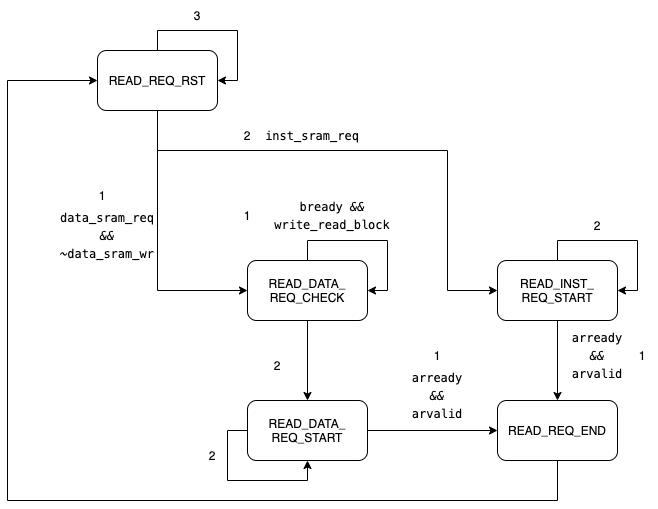
\includegraphics[width=0.6\linewidth]{figures/RREQ.png}
		\caption[rreq_status]{读请求状态转移图}
		\label{fig:rreq_status}
	\end{figure}
	
	根据需求设计状态转移图,十分清晰,当发起事务时,取指请求进入\texttt{start}状态,而数据请求进入\texttt{check}状态,若检查通过也进入\texttt{start}状态,因为是$2\times 1$的转接桥,因此这里设计两种\texttt{start}状态以便后续分别返回\texttt{addr_ok}信号,而标志接收到请求的信号组合是\texttt{arready \&\& arvalid},这种情况下表示请求一定有效,进入\texttt{end}阶段,而后直接进入\texttt{rst}复位,等待下一次请求的发起。
	
	\subparagraph{控制信号赋值逻辑}\hfill
	
	与读请求发起有关的控制信号有\texttt{ar}类输出信号,统一使用\texttt{reg}类进行时序赋值而后连接至组合逻辑输出,\texttt{arid, araddr, arsize, arvalid}对应的\texttt{reg}信号在\texttt{rreq_cur_state}或\texttt{rreq_nxt_state}处于\texttt{start}状态时即\texttt{pre_if}发起了取指请求时进行赋值即可,注意指令和数据请求分开、先考虑数据请求(避免数据还未取到被指令覆盖而后流水级往后进行)。\texttt{arvalid}信号在读请求被接受(收到\texttt{arready}的时候拉低),其他只需利用\texttt{rreq_cur_state}进行状态判断即可。
	
	\paragraph{读数据返回状态机}\hfill
	
	\subparagraph{状态设置}\hfill
	
	采用\texttt{rdata_cur_state}表示当前状态,\texttt{rdata_nxt_state}表示下一状态。
	
	\begin{center}
	\begin{tabular}{|c|c|c|}
	\hline
  	\textbf{状态} & \textbf{One-hot编码} & \textbf{解释} \\
  	\hline
	READ_DATA_RST & 3'b001 & 读数据返回处理复位 \\
	\hline
	READ_DATA_START & 3'b010 & 读数据处理开始,等待数据返回 \\
	\hline
	READ_DATA_END & 3'b100 & 读数据返回 \\
	\hline
	\end{tabular}
	\end{center}
	
	\subparagraph{状态转移图}\hfill
	
	\begin{figure}[h]
		\centering
		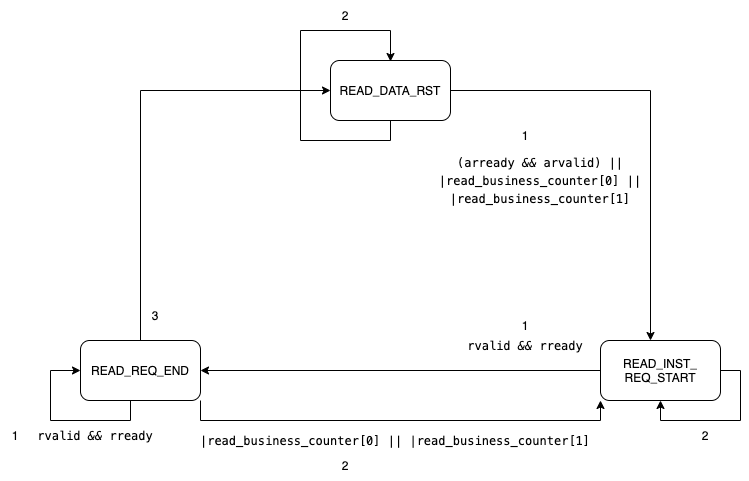
\includegraphics[width=0.75\linewidth]{figures/RDATA.png}
		\caption[rreq_status]{读返回处理状态转移图}
		\label{fig:rreq_status}
	\end{figure}
	
	这里初次设计可能会有问题,如果只按照上面读请求的简单设计,由于AXI协议强大的事务处理功能,在访存类指令来临时将面对巨量的数据请求操作。事实上,将读请求和读数据分为两个状态机的意义也在此,AXI的思想在于拆分事务,使他我们能够单独进行运作,请求和处理是不完全分开的两种事务,读写也是,将事物拆分后效率将变高。以上叙述用清晰的语言来说就是,读数据如果收到了ok信号,它真的可以直接返回复位等待吗?答案显然是未必可以,需要判断是否还有未处理完的请求事务,如果请求仍然有效,那么就继续回到处理准备\texttt{start}阶段,等待数据返回。
	
	那么问题的关键在于计算当前请求事务的数量,即可使用一个计数器counter,在每次申请成功时加一,在处理完一件事物时减一,根据计数器是否为0来判断是否还有请求事务。
	
	\subparagraph{控制信号赋值逻辑}\hfill
	
	这里控制信号是slave$\rightarrow$master的,因此无需赋值,只是由于时序需要,未来在\texttt{data_ok}信号拉高的时候判断是指令RAM还是数据RAM的时候,将\texttt{rid}暂存一拍。
	
	\paragraph{写请求状态机}\hfill
	
	\subparagraph{状态设置}\hfill
	
	采用\texttt{wrd_cur_state}表示当前状态,\texttt{wrd_nxt_state}表示下一状态。
	
	\begin{center}
	\begin{tabular}{|c|c|c|}
	\hline
  	\textbf{状态} & \textbf{One-hot编码} & \textbf{解释} \\
  	\hline
	WRITE_RST & 4'b0001 & 写请求复位 \\
	\hline
	WRITE_CHECK & 4'b0010 & 写请求检查,当前是否有读请求处于读后写相关 \\
	\hline
	WRITE_START & 4'b0100 & 写请求开始申请,等待写请求握手 \\
	\hline
	WRITE_RD_END & 4'b1000 & 写请求被接收 \\
	\hline
	\end{tabular}
	\end{center}
	
	\subparagraph{状态转移图}\hfill
	
	\begin{figure}[h]
		\centering
		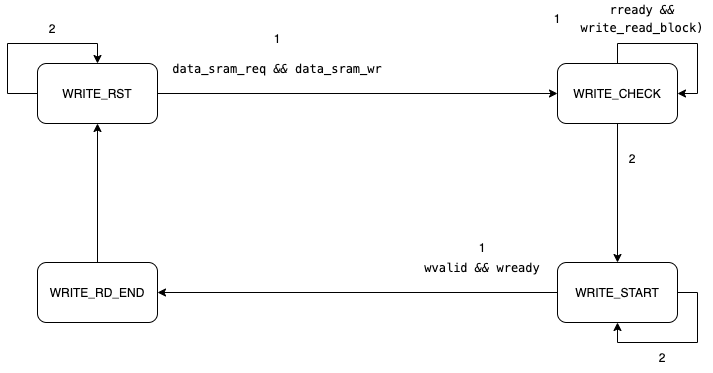
\includegraphics[width=0.75\linewidth]{figures/WRD.png}
		\caption[rreq_status]{写请求状态转移图}
		\label{fig:rreq_status}
	\end{figure}
	
	和读类似,但是这里按照讲义说法,事实上高效的AXI协议写请求还要分为两个事务:写请求(aw)和写数据请求(w),前者握手时决定写id、地址、长度、突发传输等基本配置信息,而真正要写的数据放在写数据请求。也就是说,根据AXI协议这两个事务也是(不完全)分开的,允许前者持续进行同时后者无关系地也持续进行,只要对同一写id进行准备好就能够完成写入,甚至完全可以出现后者领先前者的不符合直觉的情况。
	
	这里因为不需要如此高效,保证正确性的需要,将二者合二为一,事实上经过实践发现写数据请求握手不会在写请求握手之前出现,但可能会在之后出现,因此要准备好这种情况,简单而言,以写数据完成的握手为标准来更新\texttt{wrd_nxt_state}即可。保险起见,可以将先完成的用\texttt{reg}信号保存,后来者见到高的\texttt{reg}信号即可明白写请求已经完成握手,数据和地址等信息都已成功一起传输。
	
	再有,讲义没有提到但有可能发生的是,由于读写分开,可能出现读后写相关的错误,读请求在写请求之前发出,但写完成发生在读完成之前,这就导致读出的数据可能已经被写入,因此还需要一个检查操作。
	
	\subparagraph{控制信号赋值逻辑}\hfill
	
	控制信号在\texttt{start}状态拉高即可,\texttt{valid}信号在slave的\texttt{ready}信号到来之时拉低,其余根据状态机直接判断即可。
	
	\paragraph{写响应状态机}\hfill
	
	\subparagraph{状态设置}\hfill
	
	采用\texttt{wresp_cur_state}表示当前状态,\texttt{wresp_nxt_state}表示下一状态。
	
	\begin{center}
	\begin{tabular}{|c|c|c|}
	\hline
  	\textbf{状态} & \textbf{One-hot编码} & \textbf{解释} \\
  	\hline
	WRITE_RESPONSE_RST & 3'b001 & 写响应复位 \\
	\hline
	WRITE_RESPONSE_START & 3'b010 & 写响应开始准备,等待握手 \\
	\hline
	WRITE_RESPONSE_END & 3'b100 & 写收到响应 \\
	\hline
	\end{tabular}
	\end{center}
	
	\subparagraph{状态转移图}\hfill
	
	\begin{figure}[h]
		\centering
		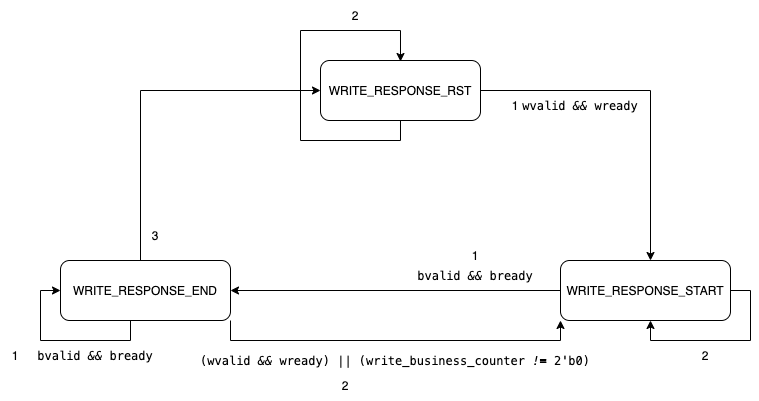
\includegraphics[width=0.75\linewidth]{figures/WRESP.png}
		\caption[rreq_status]{写响应状态转移图}
		\label{fig:rreq_status}
	\end{figure}
	
	和读响应类似,同样使用事务统计的观念去安排状态转换,若还有未完成的事务则继续等待握手。

	\subsection{除法器优化}
	
	\subsubsection{问题与改进}
	
	在和老师进行探讨之后,发现之前的设计使用的资源开销太大,之前使用了一个$32\times 64$和$32\times 32$位数组,迭代方式是叠加\texttt{reg}与\texttt{wire},每一拍用当前\texttt{wire}输出赋值下一个\texttt{reg}输入。
	
	改进方法是都只使用一个64位和32位数组,每次都去利用时序逻辑从\texttt{wire}向\texttt{reg}赋值,而后再利用\texttt{reg}进行固定的组合逻辑运算,自动更新\texttt{wire}。
	
    \begin{minted}{verilog}
    // 根据wire更新的reg
    if(reset || complete) begin
        A_r <= 64'b0;
    // 进行直接移位以优化
    end else if(skip_cal_finish && ~skipped) begin
        A_r <= (A << skip_pos);
    // 用clear_window清除对应位而后新值
    end else begin
        A_r <= ((A_r & ~clear_window) | new_A) << 1;
    end
    // 被减数
    assign minuend = A_r[63:31];
    // 减法结果
    assign minus_res = minuend - B;
    // 这次减法的商
    assign s = ~minus_res[32];
    // 是否更新被除数
    assign new_A[63:31] = s ? minus_res : minuend;
    assign new_A[30: 0] = 31'b0;
    // 余数
    assign R = A_r[63:32];
    \end{minted}
	
	事实上按照正常思路,滑动窗口在被除数上每拍右移,而若反过来思考,固定滑动窗口为高33位,那么只需要被除数每次左移,而且更新的被除数永远只在高33位赋值,写法十分方便。
	
	\subsubsection{拆分流水化}
	
	因为此前WNS较差,考虑将一拍完成的组合逻辑在中间用\texttt{reg}间隔一下,两拍完成组合逻辑赋值,于是进入除法器后查找位置操作变成2拍,而后经过只需要最少2拍的减法器,得到结果,这样外部流水线的设计就可以是在减法倒数第二拍\texttt{es}可以更新、流向\texttt{ms},最后运算完后可以直接从\texttt{ms}流走,这样是较为符合性能需要的。
	
	\section{实验过程}
	
	\subsection{实验流水账}
	
	2021.10.28 09:00 $\sim$ 2021.10.29 23:00 :尝试不使用“只在\texttt{fs_allow_in}的情况下发取指请求”的思路但失败
	
	2021.11.01 09:00 $\sim$ 2021.11.01 14:00 :Lab10初步完成,但是异常处理有bug
	
	2021.11.09 13:30 $\sim$ 2021.11.09 18:00 :Lab11初步完成,但是异常处理有bug
	
	2021.11.09 18:00 $\sim$ 2021.11.09 20:30 :解决异常处理
	
	2021.11.10 09:00 $\sim$ 2021.11.10 12:00 :运用事务处理观念解决随机延迟下此前的漏洞
	
	2021.11.11 15:30 $\sim$ 2021.11.12 10:00 :撰写实验报告
	
    2021.11.11 15:00 $\sim$ 2021.11.14 24:00(间断) :上板出现问题并解决
    
	\subsection{错误记录}	
	\subsubsection{错误\textbf{1:}频繁发请求}
	
	\paragraph{错误\textbf{1.1:}取指请求}\hfill
	
	\subparagraph{错误现象}\hfill
	
	经常出现在\texttt{fs_allow_in}被阻塞的情况下,若持续发请求,无论多大的缓冲区暂存都不够。\texttt{branch}的处理也较为复杂
	
	\begin{figure}[h]
		\centering
		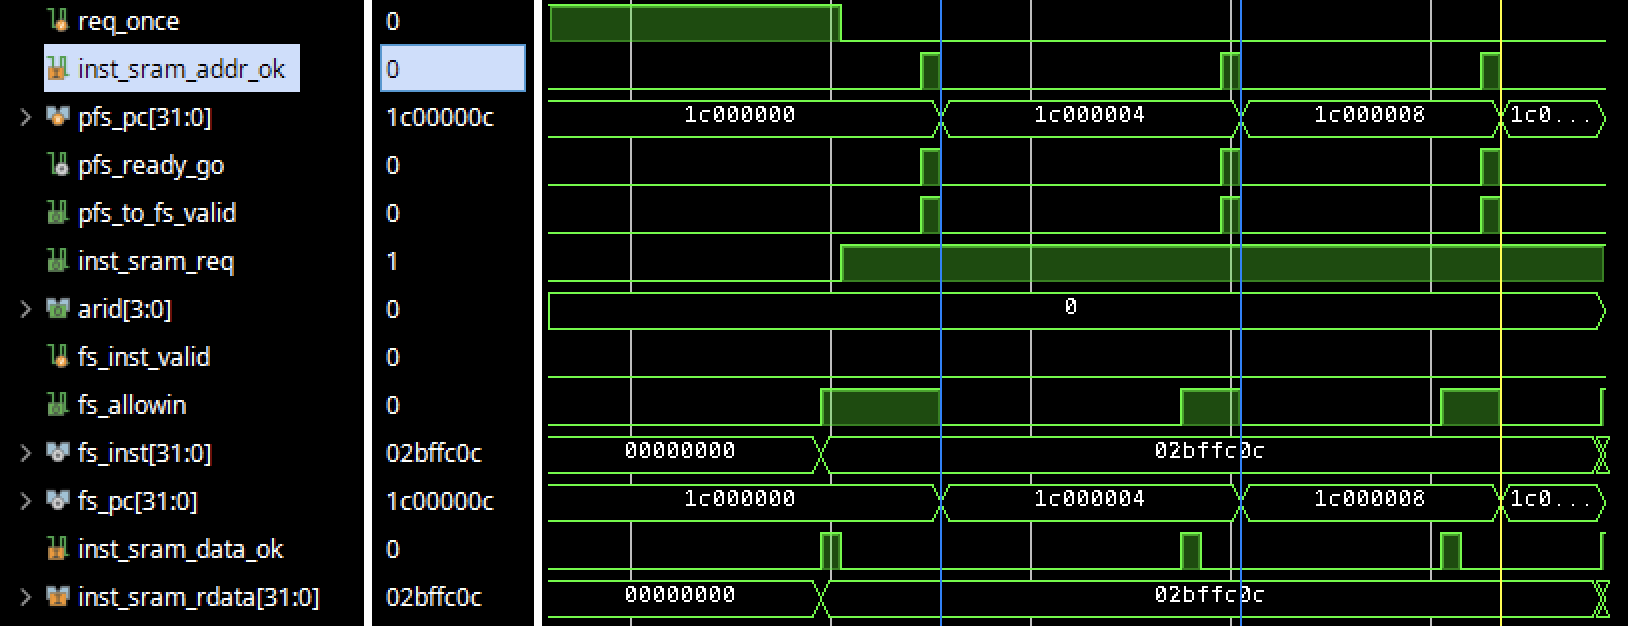
\includegraphics[width=0.85\linewidth]{inst_req_frequently.png}
		\caption[inst_req_frequently]{取指请求发送过于频繁}
		\label{fig:inst_req_frequently}
	\end{figure}
	
	\subparagraph{修正效果}\hfill
	
	只需要在\texttt{fs_allow_in}的条件下发送取指请求即可
	
    \begin{minted}{verilog}
    assign inst_sram_req = pfs_valid && fs_allowin & ~(pfs_reflush);
    \end{minted}
	
	\paragraph{错误\textbf{1.2:}数据请求}\hfill
	
	\subparagraph{错误现象}\hfill
	
	这一错误只在Lab12随机情况下出现,最离奇的错误是\texttt{load}和\texttt{store}指令同时返回成功结果,但是\texttt{data_sram_data_ok}在原先的设计中只能拉高一拍,这就引发了笔者如前的思考,错误如图:
	
	\begin{figure}[h]
		\centering
		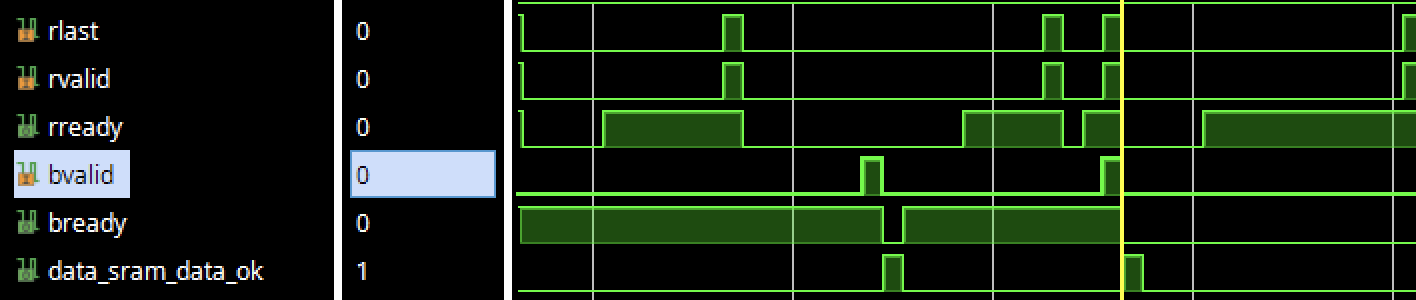
\includegraphics[width=0.8\linewidth]{data_req_frequently.png}
		\caption[data_req_frequently]{数据请求发送过于频繁}
		\label{fig:data_req_frequently}
	\end{figure}

	\subparagraph{修正效果}\hfill
	
	如同前面指令请求的处理一样,当且仅当\texttt{ms_allow_in}的时候发送数据请求。
	
	\subparagraph{总结归纳}\hfill
	
	建议讲义以后在处理这个问题的时候不要提第一种建议(即使用缓冲区存),统一按照下一级有效的时候进行请求,能够节省大量时间。在思考设计的时候也要想清楚所有可能的情况,包括特殊情况,或许还是由于对于AXI协议此前不够理解何谓读写通道分开,这样有什么结果,才导致如此的设计错误。
	
	\subsubsection{错误\textbf{2:}未使用事务处理观念弥补状态机状态转移条件}
	\label{business}
	
	\subparagraph{错误现象}\hfill
	
	经常出现对这种\texttt{load}指令,当数据RAM读数据返回了仍然有指令RAM的请求未完成的时候状态机不去等待指令RAM的返回,即下一拍\texttt{rlast, rvalid}都有效的时候却不\texttt{rready},因此导致指令不被接受,流水线卡住不继续进行。
	
	\begin{figure}[h]
		\centering
		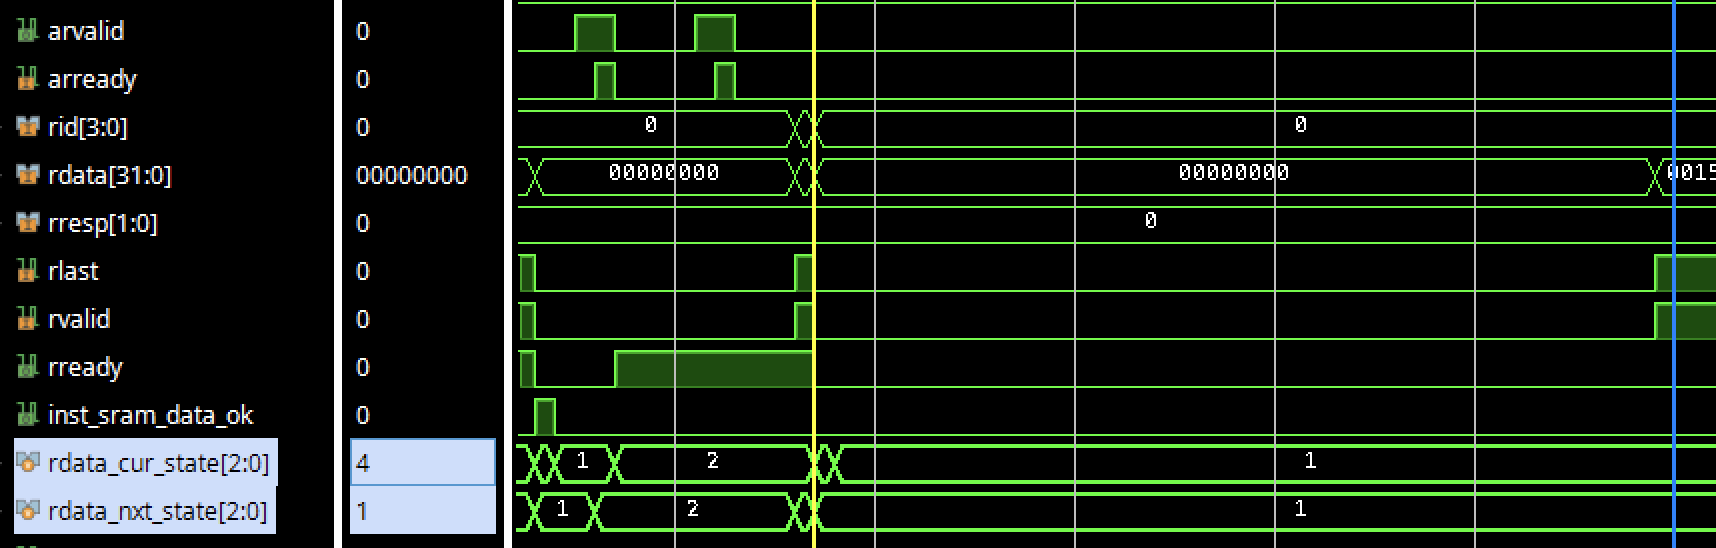
\includegraphics[width=0.8\linewidth]{rdata_business.png}
		\caption[rdata_business]{未使用事务处理弥补读响应状态机}
		\label{fig:rdata_business}
	\end{figure}
	
	写处理也是一样,在写请求密集的时候不能简单的在处理完一个请求的时候返回复位状态,要“时刻准备着”。
	
	\begin{figure}[h]
		\centering
		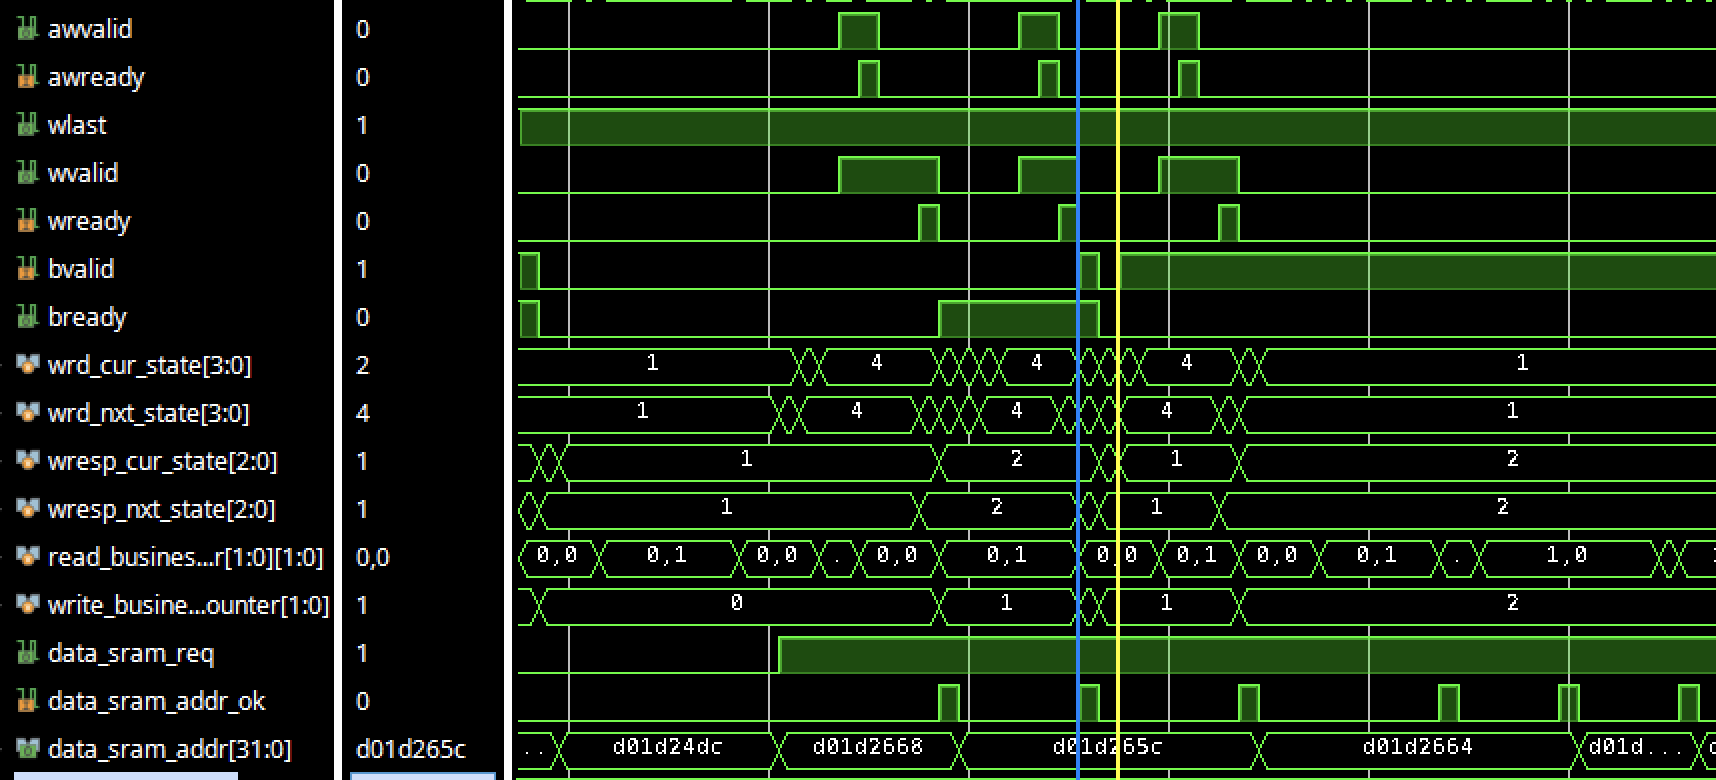
\includegraphics[width=0.8\linewidth]{wdata_business.png}
		\caption[wdata_business]{未使用事务处理弥补写响应状态机}
		\label{fig:wdata_business}
	\end{figure}
	
	\subparagraph{修正效果}\hfill
	
	修正方法如前面设计所述,添加计数器,每当收到请求时加一,请求结果返回时减一。
	
	\subparagraph{总结归纳}\hfill
	
	需要对AXI总线协议有一定的理解才能够提前想到这种可能情况,
	
	\subsubsection{错误\textbf{3:}异常处理错误}
	
	这部分错误相当密集,在此用文字进行分析和反思。根本原因是未能厘清思路便开始动笔,针对出现bug的“特殊情况”进行调试,带来时间的巨量消耗,而且出现bug有时候可能是设计疏漏但更多时候是设计错误。
	
	在早先的设计中,未能想清楚刷流水的需求,甚至对每一级刷流水的处理都不相同,这显然是不符合理论和美学的;而后没能想清楚精确异常的需求,对\texttt{load, store}指令没有特殊处理,致使内存发生不可逆改变;对于异常处理时的取指也是相当痛苦的探索,经常会有错误指令流向下一级并且第一个正确指令未能流向下一级的错误,针对特殊情况debug的后果就是,如果exec执行正常,ertn就不正常,如果解决了ertn的问题,前面的exec执行又不成功,执行反而到不了ertn。
	
	最后实在受不了这种debug思路,决定重新规划异常处理的思路,按照原理进行推演了之后既简洁美观又合情合理,编程过程简化,而且还没有bug。
	
	今后一定要坚持code after thinking的思路,在复杂问题环境下要先通过思考理清楚各种简单小case,而后再动手写代码,遇到bug要先想自己的设计是不是有原理上的错误,而后再去考虑是否是可复现、理论性的特殊情况需要进行generalize的特殊处理(比如运用读写事务处理错误2(\ref{business}))。
    	
   	\subsubsection{错误\textbf{4:}上板错误}
    	
    \paragraph{错误现象}\hfill
    
    在仿真成功、综合实现与比特流均未发生错误的情况下,上板失败,数码管在00位置卡住不动。
    
    \paragraph{错误原因}\hfill
    
    讲义上提到的错误可能有:
    
    1. 多驱动。
    
    2. 模块的 input/output 端口接入的信号方向不对。
    
    3. 时钟复位信号接错。
    
    4. 代码不规范,阻塞赋值乱用,always 语句随意使用。
    
    5. 仿真时控制信号有 “X”。仿真时,有 “X” 调 “X”,有 “Z” 调 “Z”。特别要注意的是,设计的顶层接口上不要出现 “X” 和 “Z”。
    
    6. 时序违约。
    
    7. 模块里的控制路径上的信号未进行复位。
    
    在最初的一段时间的尝试中,笔者仔细检查,1)并没有多驱动、综合也没有报错,只可能在同一个\texttt{always}块中对多个时序逻辑赋值,不可能在多个\texttt{always}块中对一个时序逻辑赋值,本身在代码形成之初就非此类设计;2)模块与新加入的模块I/O都是本就经过慎之又慎的考虑,也未出错;3)时钟复位信号有以下几套:\texttt{aresetn}和\texttt{areset},\texttt{resetn}和\texttt{reset},\texttt{rst}和\texttt{rstn},在细心一点的赋值之后基本和原来一致,原CPU使用的是\texttt{reset},即高电平有效,而新加入的AXI使用的是\texttt{aresetn}是低电平有效,这样一想之后很容易正确赋值,不构成问题;4)这更不可能,自认为代码规范性上可谓一流(\textsl{但事实证明正是由于这一点错误,人不能过于自信}),在普通的时序赋值不会有错;6)时序不可能有问题,经过大量的流水线优化以及成乘除法器自主化,对于流水时序控制已经到了相当强的力度,由实现布局布线的结果,大概WNS在5.407ns(4$\sim$7ns附近横跳)左右)针对这个确实做了一些优化,对所有\texttt{always}块里的\texttt{reg}型变量统一进行初始化、并且删除了大量的冗余信号,最后使得除了regfile寄存器堆中的未初始化寄存器之外所有信号都得到复位,几乎见不到X和Z信号的出现。
    
    在经过上述的诸多痛苦尝试后仍然有问题,咨询助教,助教推荐了使用chipscope的上板调试手段,在综合阶段进行set up debug,讲上板要抓取的信号进行记录,汇总至debug core上,然后再进行实现和比特流烧录,在上板时候就可以通过chip scope中抓取展示的相关信号进行debug。笔者看到的有问题的信号有两个(因为可以抓取的信号并不够多,但足以说明确实有问题),一个是\texttt{arvalid_r1}的信号,笔者最初以为它就是\texttt{arvalid_r},但是它在复位的时候是高电平,正常运转的时候是低电平,完全相反,令人迷惑,对于布局布线之后的一些“中间信号”还需要老师更详细地介绍,平常在看WNS最长路径的时候也很迷惑这个信号的作用是什么,为什么笔者在笔者的模块里并没有找到对应的信号;还有一个\texttt{pfs_pc}信号,它在复位期间是正常的\texttt{32'h1bfffffc},但是在运转的时候就变成了\texttt{32'b0,32'b4}之间反复横跳。
    
    这两个错误令人迷惑,也不知道从何处抓手,笔者决定重新检查状态机写法,上网搜索了三段式状态机写法,感觉未能找到类似笔者的写法:\texttt{next_state = next_state},本意是让它保持在原先的状态不变,但是应该是不符合规范的,如果在\texttt{always (*)}块中时使用这种阻塞式写法,\texttt{next_state}并不知道自己该赋给自己什么值,因为可以将这种赋值方法下\texttt{next_state}看作一种提前性的随机而变的下一状态,因此对它的赋值都必须是确定的。
    
    最终在更正了状态机的这种写法后,完成本次实验全部内容。
	
	\section{实验总结}
	
	AXI和SRAM对于我们的时序逻辑设计有着相当大的帮助,更加深入地理解了流水线各个流水级之间的交互关系,并且能够灵活为各种时序需求匹配流水线控制信号。此外,对于bug和异常的处理也让我们收获了很多宝贵的人生(计算机从业)经验。从这次试验完成,CPU与外部链接的窗口已经开启,CPU内部已经初具稳定规模,下面就可以考虑高性能设计和外部通路。
    
    本次实验完成后WNS为5.407ns。
	
\end{document}